\documentclass[a4paper,11pt]{article}

\usepackage{amsmath,amssymb,amsfonts}
\usepackage{booktabs}
\usepackage[dvipsnames]{xcolor}
\usepackage[margin=30mm]{geometry}
\usepackage{graphicx}
	\graphicspath{
		{graphics/}
	}
\usepackage{hyperref}
	\hypersetup{
		colorlinks=true,
		linkcolor=blue,
		filecolor=blue,
		urlcolor=blue,
		citecolor=blue
	}
%\usepackage[sort&compress]{natbib}
%	\bibliographystyle{apalike}
\usepackage{soul}
\usepackage{url}


% Damien added packages
\usepackage{listings}
\lstset{language=R,
    basicstyle=\small\ttfamily,
    stringstyle=\color{DarkGreen},
    otherkeywords={0,1,2,3,4,5,6,7,8,9},
    morekeywords={TRUE,FALSE},
    deletekeywords={data,frame,length,as,character},
    keywordstyle=\color{blue},
    commentstyle=\color{DarkGreen},
}
\usepackage{float}

\newcommand{\jwj}[1]{{\color{red}{~(jwj: #1)}}}
\newcommand{\yourInitials}[1]{{\color{blue}{~(yourInitials: #1)}}}

\usepackage{titlesec}
\titleformat{\section}{\normalfont\large\bfseries}{}{0pt}{}
\titleformat{\subsection}{\normalfont\large\bfseries}{}{10pt}{}
\titleformat{\subsubsection}{\normalfont\small\bfseries}{}{30pt}{}


%=======================================

\title{BOZ780 Assignment 1}
\author{DS de Gouveia \\ 15003079}
\date{\today}

\begin{document}
\maketitle
\tableofcontents

\newpage

\section{Question 1}
Dashed lines represent $z_1=5x_1-x_2$, dotted lines represent $z_2=x_1+4x_2$ and the feasible region, bounded by solid black lines is shaded gold. The co-ordinate grid in proceeding figures is represented as $(x_2,x_1)$, please take note of the axis.
\subsection{Question 1 (a): Graphical solution}
The solution to $z_2$ occurs at $(5,0)$ where the solution for $z_1$ occurs at $(0,4)$ both indicated in turquoise. These points do not coincide.
\begin{figure}[H]
    \centering
    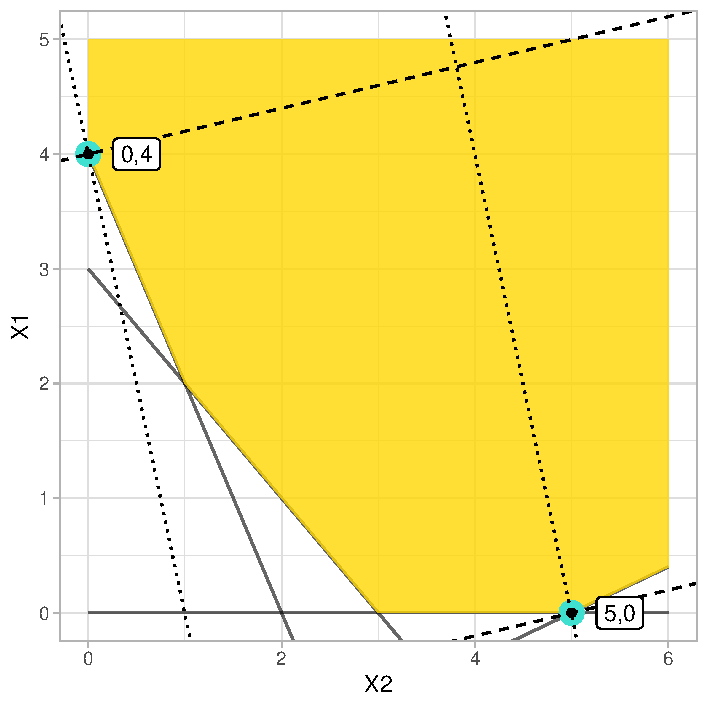
\includegraphics{../R/Optimal_points_Z1_Z2}
    \caption{Optimal points of $z_1$ and $z_2$ are not located at the same position as the gradient of their respective objective functions are tangential to each other.}
    \label{eff_front}
\end{figure}
\newpage

\subsection{Question 1 (b): Define points}
Points are defined as efficient if there is no area below the intersection of $z_1$ (dashed) and $z_2$ (dotted) that lies within the feasible region.
\begin{enumerate}
	\item $(5,0)$ Efficient
	\item $(2,1)$ Efficient
	\item $(1,1)$ Infeasible
	\item $(1,2)$ Efficient
	\item $(0,5)$ Dominated
\end{enumerate}

Point $(0,5)$ is dominated as point $(0,4)$ improves on the solution without degrading either objective.

\begin{figure}[H]
    \centering
    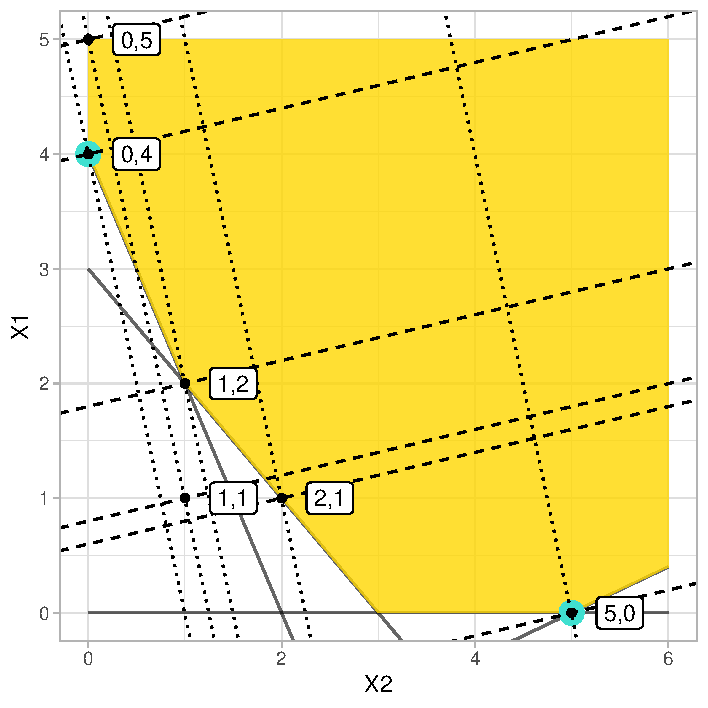
\includegraphics{../R/Efficient_dominated_other_points}
    \caption{Efficient, dominated and other points}
    \label{eff_front}
\end{figure}


\newpage
\subsection{Question 1 (c): Pre-emptive}
\subsubsection{Minimise $z_1$}
The solution found for $z_1$ is introduced as a constraint reducing the solution in which $z_2$ will attempt to find an efficient point in.
\begin{align}
	\quad \min z_1 = 5x_1 - x_2
\end{align}

Subject to:

\begin{align}
	-5x_1 + 2x_2 \leq 10\\
	x_1 + x_2 \geq 3\\
	x_1 + 2x_2 \geq 4\\
	x_1,x_2 \geq 0
\end{align}

\begin{align}
	z_1 = -5 \\
	x_1 = 0 \\
	x_2 = 5
\end{align}

\begin{figure}[H]
    \centering
    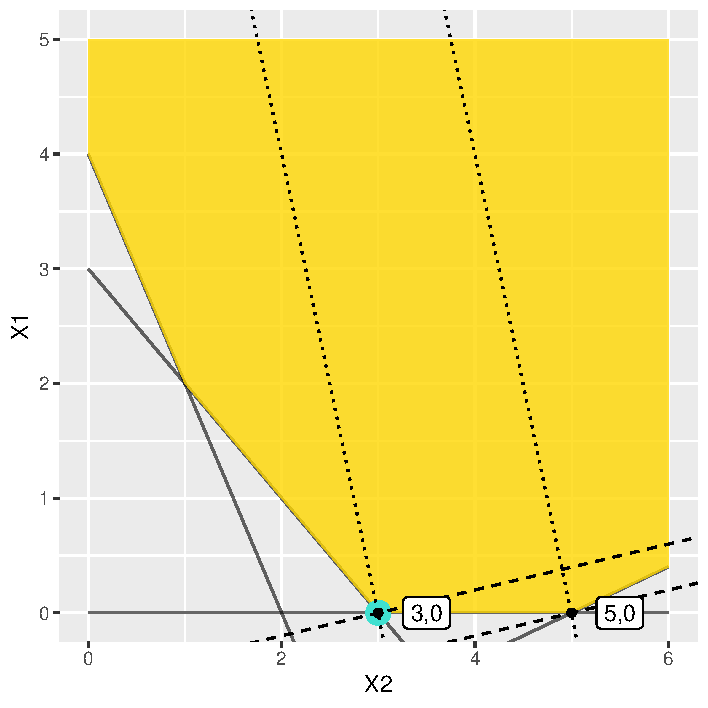
\includegraphics{../R/Pre_emptive}
    \caption{Pre-emptive feasible region with $z_1$ optimal point at $(5,0)$.}
    \label{eff_front}
\end{figure}

\subsubsection{Minimise $z_2$}

\begin{align}
	\quad \min z_2 = x_1 + 4x_2
\end{align}

Subject to:

\begin{align}
	5x_1 - x_2 \leq -5\\
	-5x_1 + 2x_2 \leq 10\\
	x_1 + x_2 \geq 3\\
	x_1 + 2x_2 \geq 4\\
	x_1,x_2 \geq 0
\end{align}

\begin{align}
	z_2 = 12 \\
	x_1 = 0 \\
	x_2 = 3
\end{align}

\begin{figure}[H]
    \centering
    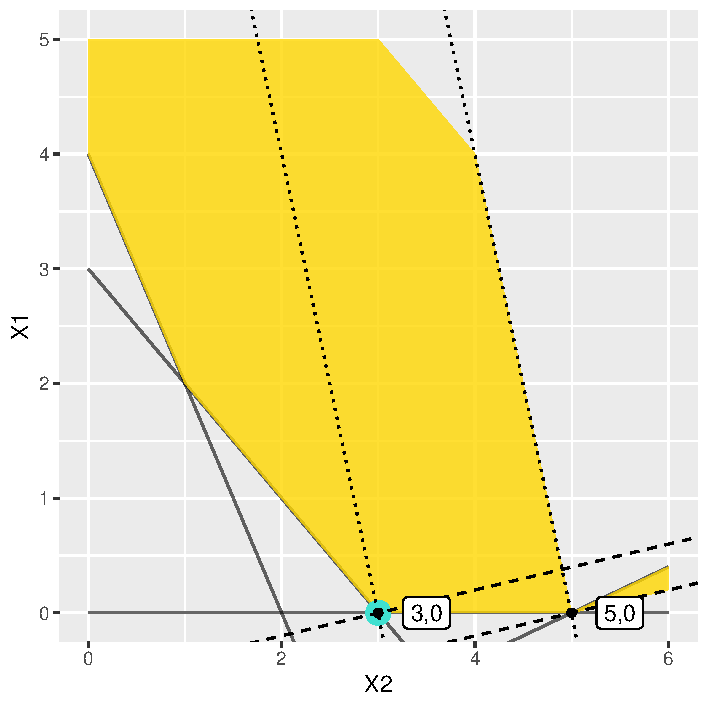
\includegraphics{../R/Pre_emptive2}
    \caption{Pre-emptive feasible region including $z_1$ constraint with $z_2$ efficient point at $(3,0)$}.
    \label{eff_front}
\end{figure}


\newpage
\subsection{Question 1 (d): Efficient frontier}
\begin{figure}[H]
    \centering
    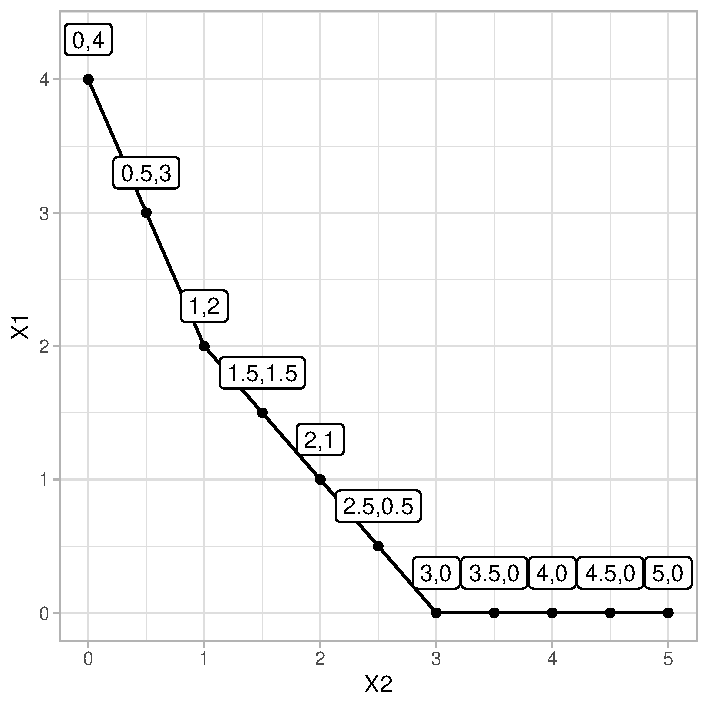
\includegraphics{../R/Efficient_frontier}
    \caption{Efficient frontier for $x_1$ and $x_2$ in increments of $0.5$}
    \label{eff_front}
\end{figure}













\newpage
\section{Question 2}
The following assumptions apply to Question 2:
\begin{itemize}
	\item The area required for a golf facility is stated as $62 \ 0000$ which exceeds the maximum area for site 1 and site 6. The lack of a thousand separator ($620 \ 000$) and a large deviation from other sites indicates this may be a potential typo. A value of $62 \ 000$ has been used instead.
	\item Weights have been stated as 1000:10:1 which is assumed to reference P1:P2:P3 as priority one to three.
\end{itemize}
\subsection{Question 2 (a) - General formulation}

\subsubsection{Sets}

\begin{tabular}{ll}
$I$ & set of facility types $I \in (1,\dots,4)$ as (Golf, Swimming, Gymnasium, Tennis)\\
$J$ & set of sites $J \in (1,\dots, 6)$ 
\end{tabular}\\

\subsubsection{Parameters}

\begin{tabular}{lll}
$d_{ij}$ & \text{user days for facility $i$ on site $j$} & $i \in I, j \in J$\\
$a_{j}$ & \text{available land on site $j$ in ft$^2$} &  $j \in J$\\
$c_{i}$ & \text{construction cost for facility $i$ in \$} & $i \in I$\\
$r_{i}$ & \text{required land for facility $i$ in ft$^2$} & $i \in I$
\end{tabular}\\


\subsubsection{Variables}

\begin{tabular}{lll}
$x_{ij}$ & 
	$\begin{cases} 
      	1 & \text{facility $i$ is built on site $j$} \\
      	0 & \text{if else} 
	\end{cases}$ & $i \in I, j \in J$
\end{tabular}\\

\setcounter{equation}{0}	

\subsubsection{Objectives}

\begin{align}
\min \quad & \sum_{i\in I} \sum_{j\in J} x_{ij}c_i & \text{(construction cost)} \\
\label{q2a.unsedlandeq}
\min \quad \sum_{j\in J}a_j - & \sum_{i\in I} \sum_{j\in J} x_{ij}r_i  & \text{(unused land cost)} \\
\max \quad & \sum_{i\in I} \sum_{j\in J} x_{ij}u_{ij}  & \text{(user days)} 
\end{align}

\subsubsection{Constraints}

\begin{align}
\sum_{i\in I} x_{ij}r_i &\leq a_j && \forall j\in J & \text{(land capacity)}        \\
x_{i1}+x_{i6} &= 0  && \forall i \in (2,3,4)  & \text{(no facilities on site 1 and 6)}\\
x_{1j} &= 0 && \forall j\in (2,3,4,5) & \text{(no golf on site 2 to 4)}\\
x_{11} + x_{16} &\leq 1 && & \text{(either site 1 or 6 can build golf)}
\end{align}

\newpage
\subsection{Question 2 (b) - Basic goal programming}
\subsubsection{Sets}
\begin{tabular}{lll}
	$K$ & set of objectives $K \in (1,2,3)$\\
	$I$ & set of facility types $I \in (1,\dots,4)$ as (Golf, Swimming, Gymnasium, Tennis)\\
$J$ & set of sites $J \in (1,\dots, 6)$ 
\end{tabular}

\subsubsection{Parameters}

\begin{tabular}{lll}
$d_{ij}$ & \text{user days for facility $i$ on site $j$} & $i \in I, j \in J$\\
$a_{j}$ & \text{available land on site $j$ in ft$^2$} &  $j \in J$\\
$c_{i}$ & \text{construction cost for facility $i$ in \$} & $i \in I$\\
$r_{i}$ & \text{required land for facility $i$ in ft$^2$} & $i \in I$
\end{tabular}\\


\subsubsection{Variables}

\begin{tabular}{lll}
$x_{ij}$ & 
$	\begin{cases} 
      	1 & \text{facility $i$ is built on site $j$} \\
      	0 & \text{if else} 
	\end{cases}$ & $i \in I, j \in J$\\
$d_k$ & deficiency variable for objective $k$ & $k\in K$
\end{tabular}

\subsubsection{Objectives}

\begin{align}
\min \quad & \sum_{k\in K} d_k & \text{(deficiencies)}
\end{align}
\subsubsection{Constraints}

\begin{align}
	\begin{split}
		\sum_{j\in J}a_j-\sum_{i\in I} \sum_{j\in J} x_{ij}r_i -d_1 & \leq 40\ 000\ \text{ft}^2 \\
		\sum_{i\in I} \sum_{j\in J} x_{ij}r_i +d_1 & \geq \sum_{j\in J}a_j -40\ 000\ \text{ft}^2  \quad \text{(P1: unused land cost)} \\
	\end{split}
\end{align}

\begin{align}
 \sum_{i\in I} \sum_{j\in J} x_{ij}c_i - d_2& < \$1.2\  \text{million} & \text{(P2: construction cost)} \\
\sum_{i\in I} \sum_{j\in J} x_{ij}u_{ij} +d_3 & \geq 200\ 000\ \text{days}  & \text{(P3: user days)} 
\end{align}
\begin{align}
\sum_{i\in I} x_{ij}r_i &\leq a_j && \forall j\in J & \text{(land capacity)}        \\
x_{i1}+x_{i6} &= 0  && \forall i \in (2,3,4)  & \text{(no facilities on site 1 and 6)}\\
x_{1j} &= 0 && \forall j\in (2,3,4,5) & \text{(no golf on site 2 to 4)}\\
x_{11} + x_{16} &\leq 1 && & \text{(either site 1 or 6 can build golf)}
\end{align}

\subsubsection{Solution}

\begin{center}
	\begin{tabular}{l c c}
		\hline
		\hline
		\textbf{Metric} & \textbf{Value} & \textbf{Target}\\
		\hline
		\hline
		Unused land & 234\ 000\ ft$^2$ & 40\ 000\ ft$^2$\\
		Used land & 271\ 000\ ft$^2$ & -\\
		Construction cost & \$\ 980\ 000 & \$\ 1\ 200\ 000 \\
		User days & 148\ 000\ days & 200\ 000\ days\\
		\hline
	\end{tabular}
\end{center}

\begin{align}
x_{ij} &= 
	\begin{bmatrix} 
    1  &  0  &  0  &  0  &  0  &  0 \\
    0  &  0  &  0  &  1  &  0  &  0 \\
    0  &  0  &  0  &  0  &  0  &  0 \\
    0  &  1  &  1  &  1  &  1  &  0 \\
	\end{bmatrix}
&d_k &= 	\begin{bmatrix} 
    194\ 000 \\
    0 \\
    52\ 000 \end{bmatrix} & \min(z) = 246\ 000
\end{align}

\newpage
\subsection{Question 2 (c) - Pre-emptive goal programming}

\subsubsection{Sets}
\begin{tabular}{lll}
	$K$ & set of objectives $K \in (1,2,3)$\\
	$I$ & set of facility types $I \in (1,\dots,4)$ as (Golf, Swimming, Gymnasium, Tennis)\\
$J$ & set of sites $J \in (1,\dots, 6)$ 
\end{tabular}

\subsubsection{Parameters}

\begin{tabular}{lll}
$d_{ij}$ & \text{user days for facility $i$ on site $j$} & $i \in I, j \in J$\\
$a_{j}$ & \text{available land on site $j$ in ft$^2$} &  $j \in J$\\
$c_{i}$ & \text{construction cost for facility $i$ in \$} & $i \in I$\\
$r_{i}$ & \text{required land for facility $i$ in ft$^2$} & $i \in I$
\end{tabular}\\


\subsubsection{Variables}

\begin{tabular}{lll}
$x_{ij}$ & 
$	\begin{cases} 
      	1 & \text{facility $i$ is built on site $j$} \\
      	0 & \text{if else} 
	\end{cases}$ & $i \in I, j \in J$\\
$d_k$ & deficiency variable for objective $k$ & $k\in K$
\end{tabular}


\subsubsection{Objectives}
\begin{align}
\min \quad & d_1 & \\
\min \quad & d_2 & \text{(subject to $d_1$)}\\
\min \quad & d_3 & \text{(subject to $d_1$ and $d_2$)}
\end{align}

\subsubsection{Constraints}

\begin{align}
& d_1=0 & \text{(used in $d_2$ and $d_3$)} \\
& d_2=0 & \text{(used in $d_3$)}
\end{align}
\begin{align}
	\sum_{i\in I} \sum_{j\in J} x_{ij}r_i +d_1 & \geq \sum_{j\in J}a_j -40\ 000\ \text{ft}^2  & \text{(P1: unused land cost)} \\
 \sum_{i\in I} \sum_{j\in J} x_{ij}c_i - d_2& < \$1.2\  \text{million} & \text{(P2: construction cost)} \\
\sum_{i\in I} \sum_{j\in J} x_{ij}u_{ij} +d_3 & \geq 200\ 000\ \text{days}  & \text{(P3: user days)} 
\end{align}
\begin{align}
\sum_{i\in I} x_{ij}r_i &\leq a_j && \forall j\in J & \text{(land capacity)}        \\
x_{i1}+x_{i6} &= 0  && \forall i \in (2,3,4)  & \text{(no facilities on site 1 and 6)}\\
x_{1j} &= 0 && \forall j\in (2,3,4,5) & \text{(no golf on site 2 to 4)}\\
x_{11} + x_{16} &\leq 1 && & \text{(either site 1 or 6 can build golf)}
\end{align}
\subsubsection{Solution: P1}
\begin{center}
	\begin{tabular}{l c c}
		\hline
		\hline
		\textbf{Metric} & \textbf{Value} & \textbf{Target}\\
		\hline
		\hline
		Unused land & 107\ 000\ ft$^2$ & 40\ 000\ ft$^2$\\
		Used land & 398\ 000\ ft$^2$ & -\\
		Construction cost & \$\ 4\ 015\ 000 & \$\ 1\ 200\ 000 \\
		User days & 277\ 000\ days & 200\ 000\ days\\
		\hline
	\end{tabular}
\end{center}

\begin{align}
x_{ij} &= 
	\begin{bmatrix} 
    1  &  0  &  0  &  0  &  0  &  0 \\
    0  &  1  &  1  &  0  &  1  &  0 \\
    0  &  1  &  0  &  1  &  1  &  0 \\
    0  &  0  &  1  &  1  &  1  &  0 \\
	\end{bmatrix}
&d_1 &= 	\begin{bmatrix} 
    67\ 000  \end{bmatrix} & \min(z) = 67\ 000
\end{align}

\subsubsection{Solution: P2}
A new constraint was included whereby $d_1 <= 67\ 000$.
\begin{center}
	\begin{tabular}{l c c}
		\hline
		\hline
		\textbf{Metric} & \textbf{Value} & \textbf{Target}\\
		\hline
		\hline
		Unused land & 107\ 000\ ft$^2$ & 40\ 000\ ft$^2$\\
		Used land & 398\ 000\ ft$^2$ & -\\
		Construction cost & \$\ 4\ 015\ 000 & \$\ 1\ 200\ 000 \\
		User days & 277\ 000\ days & 200\ 000\ days\\
		\hline
	\end{tabular}
\end{center}

\begin{align}
x_{ij} &= 
	\begin{bmatrix} 
    1  &  0  &  0  &  0  &  0  &  0 \\
    0  &  1  &  1  &  0  &  1  &  0 \\
    0  &  1  &  0  &  1  &  1  &  0 \\
    0  &  0  &  1  &  1  &  1  &  0 \\
	\end{bmatrix}
&d_2 &= 	\begin{bmatrix} 
    2\ 815\ 000 \end{bmatrix} & \min(z) = 2\ 815\ 000
\end{align}

\subsubsection{Solution: P3}
Two new constraint were included whereby $d_1 <= 67\ 000$ and $d_2 <= 2\ 815\ 000$.
\begin{center}
	\begin{tabular}{l c c}
		\hline
		\hline
		\textbf{Metric} & \textbf{Value} & \textbf{Target}\\
		\hline
		\hline
		Unused land & 107\ 000\ ft$^2$ & 40\ 000\ ft$^2$\\
		Used land & 398\ 000\ ft$^2$ & -\\
		Construction cost & \$\ 4\ 015\ 000 & \$\ 1\ 200\ 000 \\
		User days & 277\ 000\ days & 200\ 000\ days\\
		\hline
	\end{tabular}
\end{center}

\begin{align}
x_{ij} &= 
	\begin{bmatrix} 
    1  &  0  &  0  &  0  &  0  &  0 \\
    0  &  1  &  1  &  0  &  1  &  0 \\
    0  &  1  &  0  &  1  &  1  &  0 \\
    0  &  0  &  1  &  1  &  1  &  0 \\
	\end{bmatrix}
&d_3 &= 	\begin{bmatrix} 
    0 \end{bmatrix} & \min(z) = 0
\end{align}

The first priority ensured that area was maximised, inadvertently ensuring  more user days (than targeted) could occur. However, the construction cost greatly increased and with the imposed $d_1$ constraint could not decrease after the second minimisation attempt.

\newpage
\subsection{Question 2 (d) - Weighted sum goal programming}
\subsubsection{Sets}
\begin{tabular}{lll}
	$K$ & set of objectives $K \in (1,2,3)$\\
	$I$ & set of facility types $I \in (1,\dots,4)$ as (Golf, Swimming, Gymnasium, Tennis)\\
$J$ & set of sites $J \in (1,\dots, 6)$ 
\end{tabular}

\subsubsection{Parameters}

\begin{tabular}{lll}
$d_{ij}$ & \text{user days for facility $i$ on site $j$} & $i \in I, j \in J$\\
$a_{j}$ & \text{available land on site $j$ in ft$^2$} &  $j \in J$\\
$c_{i}$ & \text{construction cost for facility $i$ in \$} & $i \in I$\\
$r_{i}$ & \text{required land for facility $i$ in ft$^2$} & $i \in I$
\end{tabular}\\


\subsubsection{Variables}

\begin{tabular}{lll}
$x_{ij}$ & 
$	\begin{cases} 
      	1 & \text{facility $i$ is built on site $j$} \\
      	0 & \text{if else} 
	\end{cases}$ & $i \in I, j \in J$\\
$d_k$ & deficiency variable for objective $k$ & $k\in K$
\end{tabular}


\subsubsection{Objectives}
\begin{align}
\min \quad & 1000d_1+10d_2+d_3 
\end{align}

\subsubsection{Constraints}

\begin{align}
	\sum_{i\in I} \sum_{j\in J} x_{ij}r_i +d_1 & \geq \sum_{j\in J}a_j -40\ 000\ \text{ft}^2  & \text{(P1: unused land cost)}\\
 \sum_{i\in I} \sum_{j\in J} x_{ij}c_i - d_2& < \$1.2\  \text{million} & \text{(P2: construction cost)} \\
\sum_{i\in I} \sum_{j\in J} x_{ij}u_{ij} +d_3 & \geq 200\ 000\ \text{days}  & \text{(P3: user days)} 
\end{align}
\begin{align}
\sum_{i\in I} x_{ij}r_i &\leq a_j && \forall j\in J & \text{(land capacity)}        \\
x_{i1}+x_{i6} &= 0  && \forall i \in (2,3,4)  & \text{(no facilities on site 1 and 6)}\\
x_{1j} &= 0 && \forall j\in (2,3,4,5) & \text{(no golf on site 2 to 4)}\\
x_{11} + x_{16} &\leq 1 && & \text{(either site 1 or 6 can build golf)}
\end{align}

\subsubsection{Solution}
\begin{center}
	\begin{tabular}{l c c}
		\hline
		\hline
		\textbf{Metric} & \textbf{Value} & \textbf{Target}\\
		\hline
		\hline
		Unused land & 107\ 000\ ft$^2$ & 40\ 000\ ft$^2$\\
		Used land & 398\ 000\ ft$^2$ & -\\
		Construction cost & \$\ 4\ 015\ 000 & \$\ 1\ 200\ 000 \\
		User days & 277\ 000\ days & 200\ 000\ days\\
		\hline
	\end{tabular}
\end{center}

\begin{align}
x_{ij} &= 
	\begin{bmatrix} 
    1  &  0  &  0  &  0  &  0  &  0 \\
    0  &  1  &  1  &  0  &  1  &  0 \\
    0  &  1  &  0  &  1  &  1  &  0 \\
    0  &  0  &  1  &  1  &  1  &  0 \\
	\end{bmatrix}
&d_k &= 	\begin{bmatrix} 
    67\ 000 \\
    2\ 814\ 999\\
    0 \end{bmatrix} & \min(z) = 95\ 150\ 000
\end{align}




\newpage
\subsection{Question 2 (e) - Basic goal programming efficiency adjustment}
\subsubsection{Sets}
\begin{tabular}{lll}
	$K$ & set of objectives $K \in (1,2,3)$\\
	$I$ & set of facility types $I \in (1,\dots,4)$ as (Golf, Swimming, Gymnasium, Tennis)\\
$J$ & set of sites $J \in (1,\dots, 6)$ 
\end{tabular}

\subsubsection{Parameters}

\begin{tabular}{lll}
$d_{ij}$ & \text{user days for facility $i$ on site $j$} & $i \in I, j \in J$\\
$a_{j}$ & \text{available land on site $j$ in ft$^2$} &  $j \in J$\\
$c_{i}$ & \text{construction cost for facility $i$ in \$} & $i \in I$\\
$r_{i}$ & \text{required land for facility $i$ in ft$^2$} & $i \in I$
\end{tabular}\\


\subsubsection{Variables}

\begin{tabular}{lll}
$x_{ij}$ & 
$	\begin{cases} 
      	1 & \text{facility $i$ is built on site $j$} \\
      	0 & \text{if else} 
	\end{cases}$ & $i \in I, j \in J$\\
$d_k$ & deficiency variable for objective $k$ & $k\in K$
\end{tabular}

\subsubsection{Objectives}
A small number $0.26$ has been selected as the adjustment factor with positive and negative signs applied for minimisation and maximisation respectively.
\begin{align}
	\begin{split}
	\min \quad \sum_{k\in K}d_k &+ 0.001(\sum_{i\in I} \sum_{j\in J} x_{ij}c_i)\\
		&- 0.26(\sum_{i\in I} \sum_{j\in J} x_{ij}r_i)\\
		&- 0.26(\sum_{i\in I} \sum_{j\in J} x_{ij}u_{ij})	
	\end{split}
\end{align}
The unused area objective function (\ref{q2a.unsedlandeq}) has been converted from a minimisation of unused area to a maximisation of used area resulting in a $-0.26$ factor. The outcome of the objective is unchained and the constant $a_j$ is removed whilst the land capacity constraint prevents the area of used land from surpassing what is available.
\subsubsection{Constraints}
\begin{align}
	\sum_{i\in I} \sum_{j\in J} x_{ij}r_i +d_1 & \geq \sum_{j\in J}a_j -40\ 000\ \text{ft}^2  & \text{(P1: unused land cost)}\\
 \sum_{i\in I} \sum_{j\in J} x_{ij}c_i - d_2& < \$1.2\  \text{million} & \text{(P2: construction cost)} \\
\sum_{i\in I} \sum_{j\in J} x_{ij}u_{ij} +d_3 & \geq 200\ 000\ \text{days}  & \text{(P3: user days)} 
\end{align}
\begin{align}
\sum_{i\in I} x_{ij}r_i &\leq a_j && \forall j\in J & \text{(land capacity)}        \\
x_{i1}+x_{i6} &= 0  && \forall i \in (2,3,4)  & \text{(no facilities on site 1 and 6)}\\
x_{1j} &= 0 && \forall j\in (2,3,4,5) & \text{(no golf on site 2 to 4)}\\
x_{11} + x_{16} &\leq 1 && & \text{(either site 1 or 6 can build golf)}
\end{align}

\subsubsection{Solution}
\begin{center}
	\begin{tabular}{l c c}
		\hline
		\hline
		\textbf{Metric} & \textbf{Value} & \textbf{Target}\\
		\hline
		\hline
		Unused land & 263\ 000\ ft$^2$ & 40\ 000\ ft$^2$\\
		Used land & 242\ 000\ ft$^2$ & -\\
		Construction cost & \$\ 680\ 000 & \$\ 1\ 200\ 000 \\
		User days & 116\ 000\ days & 200\ 000\ days\\
		\hline
	\end{tabular}
\end{center}

\begin{align}
x_{ij} &= 
	\begin{bmatrix} 
    1  &  0  &  0  &  0  &  0  &  0 \\
    0  &  0  &  0  &  0  &  0  &  0 \\
    0  &  0  &  0  &  0  &  0  &  0 \\
    0  &  1  &  1  &  1  &  1  &  0 \\
	\end{bmatrix}
&d_k &= 	\begin{bmatrix} 
    223\ 000 \\
    0 \\
    84\ 000 \end{bmatrix} & \min(z) = 390\ 720
\end{align}

Including the efficiency adjustment results in the cheaper facility being built over others. The co-efficient values attributed to cost far exceed that of area and user days giving it a greater relative weight.
\newpage
\section{Question 1 R Code}
\begin{verbatim}
	library(tidyverse)
library(gridExtra)
library(lpSolve)
library(extrafont) 

### ================ Question 1 
w <- 12
h <- 12

lp(direction = "min",
   objective.in = c(1,4),
   const.mat = matrix(c(-5,1,1,0,1,
                        2,1,2,1,0),ncol = 2,byrow = FALSE),
   const.dir = c("<=",">=",">=",">=",">="),
   const.rhs = c(10,3,4,0,0))$solution


lengthX <- 6
lengthY <- 5

x <- 0:lengthX
c1 <- (x)*2/5-2
c2 <- -x +3
c3 <- -2*x+4
c4 <- rep(0,lengthX+1)

df.points <- data.frame(x=c(0,1,1,2,5,0),
                        y=c(5,2,1,1,0,4))
df.pointsOptimal <- data.frame(x=c(0,5),
                               y=c(4,0))
point.coords = paste(df.points$x,df.points$y,sep=",")
z1.intercept <- df.points$y -1/5*df.points$x
z2.intercept <- df.points$y +4 *df.points$x

# ==== Optimal points
pointOptimal.coords = paste(df.pointsOptimal$x,df.pointsOptimal$y,sep=",")
data.frame(x, c1,c2,c3,c4) %>% 
  ggplot(aes(x = x))+
  geom_line(aes(y=c1), alpha = 0.6)+
  geom_line(aes(y=c2), alpha = 0.6)+
  geom_line(aes(y=c3), alpha = 0.6)+
  geom_line(aes(y=c4), alpha = 0.6)+
  geom_ribbon(aes(ymin = pmax(c1,c2,c3,c4),
                  ymax = lengthY),
                  fill = 'gold', 
                  alpha = 0.8)+
  geom_point(data = df.pointsOptimal, aes(x=x, y=y), color = "turquoise", size = 5)+
  geom_point(data = df.pointsOptimal, aes(x=x, y=y))+
  coord_cartesian(xlim = c(0,lengthX), ylim = c(0,lengthY))+
  labs(x="X2", y="X1")+
  geom_abline(slope = 1/5, intercept = c(4,-1), linetype = "dashed", color = "black")+
  geom_abline(slope = -4, intercept = c(4,20), linetype = "dotted", color = "black")+
  geom_label(data = df.pointsOptimal,aes(x+.5,y,label=pointOptimal.coords))+
  theme_light()

ggsave("Optimal_points_Z1_Z2.pdf",dpi = "retina", width = w, height = h, units = "cm")

# === Which points are eff

data.frame(x, c1,c2,c3,c4) %>% 
  ggplot(aes(x = x))+
  geom_line(aes(y=c1), alpha = 0.6)+
  geom_line(aes(y=c2), alpha = 0.6)+
  geom_line(aes(y=c3), alpha = 0.6)+
  geom_line(aes(y=c4), alpha = 0.6)+
  geom_ribbon(aes(ymin = pmax(c1,c2,c3,c4),
                  ymax = lengthY),
              fill = 'gold', 
              alpha = 0.8)+
  geom_point(data = df.pointsOptimal, aes(x=x, y=y), color = "turquoise", size = 5)+
  geom_point(data = df.points, aes(x=x, y=y))+
  coord_cartesian(xlim = c(0,lengthX), ylim = c(0,lengthY))+
  labs(x="X2", y="X1")+
  geom_abline(slope = 1/5, intercept = z1.intercept, linetype = "dashed", color = "black")+
  geom_abline(slope = -4, intercept = z2.intercept, linetype = "dotted", color = "black")+
  geom_label(data = df.points,aes(x+.5,y,label=point.coords))+
  theme_light()
ggsave("Efficient_dominated_other_points.pdf",dpi = "retina", width = w, height = h, units = "cm")

# Question 1 c - pre-emptive

z1 <- lp(direction = "min",
   objective.in = c(5,-1),
   const.mat = matrix(c(-5,1,1,0,1,
                         2,1,2,1,0),ncol = 2,byrow = FALSE),
   const.dir = c("<=",">=",">=",">=",">="),
   const.rhs = c(10,3,4,0,0))

z2 <- lp(direction = "min",
         objective.in = c(1,4),
         const.mat = matrix(c(-5,1,1,0,1,1,0,
                               2,1,2,1,0,0,1),ncol = 2,byrow = FALSE),
         const.dir = c("<=",">=",">=",">=",">=","<=","<="),
         const.rhs = c(10,3,4,0,0,z1$solution[1],z1$solution[2]))

z1
z2
z1$solution
z2$solution

df.pointsOptimal <- data.frame(y=c(z1$solution[1],z2$solution[1]),
                               x=c(z1$solution[2],z2$solution[2]))
point.coords = paste(df.pointsOptimal$x,df.pointsOptimal$y,sep=",")
z1.intercept <- df.pointsOptimal$y -1/5*df.pointsOptimal$x
z2.intercept <- df.pointsOptimal$y +4 *df.pointsOptimal$x


data.frame(x,c1,c2,c3,c4) %>% 
  ggplot(aes(x = x))+
  geom_line(aes(y=c1), alpha = 0.6)+
  geom_line(aes(y=c2), alpha = 0.6)+
  geom_line(aes(y=c3), alpha = 0.6)+
  geom_line(aes(y=c4), alpha = 0.6)+
  geom_ribbon(aes(ymin = pmax(c1,c2,c3,c4),
                  ymax = lengthY),
              fill = 'gold', 
              alpha = 0.8)+
  geom_point(data = df.pointsOptimal[2,], aes(x=x, y=y), color = "turquoise", size = 5)+
  geom_point(data = df.pointsOptimal, aes(x=x, y=y))+
  coord_cartesian(xlim = c(0,lengthX), ylim = c(0,lengthY))+
  labs(x="X2", y="X1")+
  geom_abline(slope = 1/5, intercept = z1.intercept, linetype = "dashed", color = "black")+
  geom_abline(slope = -4, intercept = z2.intercept, linetype = "dotted", color = "black")+
  geom_label(data = df.pointsOptimal,aes(x+.5,y,label=point.coords))

ggsave("Pre_emptive.pdf",dpi = "retina", width = w, height = h, units = "cm")



#Pre-emptive with constraint from past solution
c5 <- 1/5*(x)-1
upper <- rep(lengthY, lengthX+1)


data.frame(x,c1,c2,c3,c4,c5) %>% 
  ggplot(aes(x = x))+
  geom_line(aes(y=c1), alpha = 0.6)+
  geom_line(aes(y=c2), alpha = 0.6)+
  geom_line(aes(y=c3), alpha = 0.6)+
  geom_line(aes(y=c4), alpha = 0.6)+
  geom_ribbon(aes(ymin = pmax(c1,c2,c3,c4),
                  ymax = c(5,5,5,5,4,0,0.2)),
              fill = 'gold', 
              alpha = 0.8)+
  geom_point(data = df.pointsOptimal[2,], aes(x=x, y=y), color = "turquoise", size = 5)+
  geom_point(data = df.pointsOptimal, aes(x=x, y=y))+
  coord_cartesian(xlim = c(0,lengthX), ylim = c(0,lengthY))+
  labs(x="X2", y="X1")+
  geom_abline(slope = 1/5, intercept = z1.intercept, linetype = "dashed", color = "black")+
  geom_abline(slope = -4, intercept = z2.intercept, linetype = "dotted", color = "black")+
  geom_label(data = df.pointsOptimal,aes(x+.5,y,label=point.coords))

ggsave("Pre_emptive2.pdf",dpi = "retina", width = w, height = h, units = "cm")







# Eff fronteir 

z2.seq <- seq(0,5,0.5)
df.eff <- data.frame(Obj=z2.seq, x=z2.seq, y=z2.seq)
n = 1
for (i in z2.seq){
  
  ef.front <- lp(direction = "min",
     objective.in = c(5,-1),
     const.mat = matrix(c(-5,1,1,0,1,0,
                           2,1,2,1,0,1),ncol = 2,byrow = FALSE),
     const.dir = c("<=",">=",">=",">=",">=","<="),
     const.rhs = c(10,3,4,0,0,i))
  df.eff$Obj[n] <- ef.front$objval
  df.eff$x[n] <- ef.front$solution[2]
  df.eff$y[n] <- ef.front$solution[1]
  n <- n+1
}

df.eff %>% 
  ggplot(aes(x=x, y=y))+
  geom_path()+
  geom_point()+
  labs(x="X2", y="X1")+
  geom_label(aes(x,y+.3,label=paste(x,y,sep=",")))+
  theme_light()
  
ggsave("Efficient_frontier.pdf",dpi = "retina", width = w, height = h, units = "cm")



\end{verbatim}


\newpage
\section{Question 2 R Code}
\begin{verbatim}
library(tidyverse)
library(lpSolve)
matmaker <- function(index,length){
  vec <- rep(0,length)
  vec[index] <- 1
  return(vec)
}

#======================== Q2
#=========== Parameters
i <- 4
j <- 6
k <- 3

uij <- 1000* c(31, 0, 0, 0, 0,27,
                0,25,21,32,32, 0,
                0,37,29,38,28, 0,
                0,20,23,22,20, 0)
aj <- 1000* rep(c(80,70,80,90,120,65),i)
ci <- rep(c(340000, 300000, 840000, 85000),j) %>% matrix(nrow = i, byrow = F) %>% t() %>% as.vector()
ri <- rep(c(62000 ,29000 ,38000 ,45000),j) %>% matrix(nrow = i, byrow = F)  %>% t() %>% as.vector()
dk <- c(0,0,0)

dk.k <- c(rep(0,j*i),c(1,1,1))
uij.k <- c(dij, dk)
aj.k <- c(aj, dk)
ci.k <- c(ci, dk)
ri.k <- c(ri, dk)

len <- length(ri.k)

fn.cost <- function(lpsolve.out){
   cost.landused <- sum(lpsolve.out[1:24]*ri)
   cost.landunused <- -sum(lpsolve.out[1:24]*ri) + sum(1000*c(80,70,80,90,120,65))
   cost.construction <- sum(lpsolve.out[1:24]*ci)
   cost.userdays <- sum(lpsolve.out[1:24]*uij)
   return(paste(paste("Used land",cost.landused,sep = ": "),
                paste("Unused land",cost.landunused,sep = ": "),
                paste("Construction cost",cost.construction,sep = ": "),
                paste("User days",cost.userdays,sep = ": "),sep = "       "))
}

#=========== Constraints
cons1.lhs <- c(ri.k*matmaker(c(1,7,13,19),len),
               ri.k*matmaker(c(1+1,7+1,13+1,19+1),len),
               ri.k*matmaker(c(1+2,7+2,13+2,19+2),len),
               ri.k*matmaker(c(1+3,7+3,13+3,19+3),len),
               ri.k*matmaker(c(1+4,7+4,13+4,19+4),len),
               ri.k*matmaker(c(1+5,7+5,13+5,19+5),len)) %>% matrix(nrow = 6, byrow = T)
cons1.rhs <- 1000*c(80,70,80,90,120,65)

cons2.lhs <- (rep(1,len)*matmaker(c(7,13,19,12,18,24,2,3,4,5),len))#[1:24] %>% matrix(nrow = 4, byrow = T)
cons2.rhs <- 0

cons3.lhs <- (rep(1,len)*matmaker(c(1,6),len))#[1:24] %>% matrix(nrow = 4, byrow = T)
cons3.rhs <- 1

base.cons.lhs <- rbind(cons1.lhs,cons2.lhs,cons3.lhs)
base.cons.rhs <- c(cons1.rhs, cons2.rhs, cons3.rhs)
base.cons.dir <- c(rep("<=",j), "=","<=")
#======================== Q2B
q2b.obj <- rep(1,len)*matmaker(c(27,26,25),len)

cons1.lhs <- (ri.k+dk.k*matmaker(25,len))#[1:24] %>% matrix(nrow = 4, byrow = T)
cons1.rhs <- -40000 + (1000*sum(80,70,80,90,120,65))
cons2.lhs <- ci.k-dk.k*matmaker(26,len)
cons2.rhs <- 1200000
cons3.lhs <- uij.k+dk.k*matmaker(27,len)
cons3.rhs <- 200000

q2b.cons.lhs <- rbind(base.cons.lhs, cons1.lhs, cons2.lhs, cons3.lhs)
q2b.cons.rhs <- c(base.cons.rhs, cons1.rhs, cons2.rhs, cons3.rhs)
q2b.cons.dir <- c(base.cons.dir, ">=","<",">=")

q2b.lp <- lp(direction = "min",
   objective.in = q2b.obj, 
   const.mat = q2b.cons.lhs, 
   const.rhs = q2b.cons.rhs, 
   const.dir = q2b.cons.dir, 
   binary.vec = 1:24)
q2b.lp
q2b.lp$solution[1:24] %>% matrix(nrow = i, byrow = T)
q2b.lp$solution[25:27]
q2b.lp$solution %>% fn.cost()
#======================== Q2C
#========== P1
q2c.obj.p1 <- rep(1,len)*matmaker(c(25),len)
  
q2c.lp <- lp(direction = "min",
             objective.in = q2c.obj.p1, 
             const.mat = q2b.cons.lhs, 
             const.rhs = q2b.cons.rhs, 
             const.dir = q2b.cons.dir, 
             binary.vec = 1:24)
q2c.lp
q2c.lp$solution[1:24] %>% matrix(nrow = i, byrow = T)
q2c.lp$solution[25:27] %>% as.integer()
q2c.lp$solution %>% fn.cost
#========== P2
q2c.obj.p2 <- rep(1,len)*matmaker(c(26),len)

cons1.lhs <- rep(1,len)*matmaker(25,len)
cons1.rhs <- q2c.lp$solution[25]
cons1.dir <- "<="

q2c.cons.lhs.p2 <- rbind(q2b.cons.lhs, cons1.lhs)
q2c.cons.rhs.p2 <- c(q2b.cons.rhs,cons1.rhs)
q2c.cons.dir.p2 <- c(q2b.cons.dir,cons1.dir)

q2c.lp.p2 <- lp(direction = "min",
             objective.in = q2c.obj.p2, 
             const.mat = q2c.cons.lhs.p2, 
             const.rhs = q2c.cons.rhs.p2, 
             const.dir = q2c.cons.dir.p2, 
             binary.vec = 1:24)
q2c.lp.p2
q2c.lp.p2$solution[1:24] %>% matrix(nrow = i, byrow = T)
q2c.lp.p2$solution[25:27] %>% as.integer()
q2c.lp.p2$solution %>% fn.cost()
#========== P3
q2c.obj.p3 <- rep(1,len)*matmaker(c(27),len)

cons1.lhs <- rep(1,len)*matmaker(26,len)
cons1.rhs <- q2c.lp.p2$solution[26]
cons1.dir <- "<="

q2c.cons.lhs.p3 <- rbind(q2c.cons.lhs.p2, cons1.lhs)
q2c.cons.rhs.p3 <- c(q2c.cons.rhs.p2,cons1.rhs)
q2c.cons.dir.p3 <- c(q2c.cons.dir.p2,cons1.dir)

q2c.lp.p3 <- lp(direction = "min",
                objective.in = q2c.obj.p3, 
                const.mat = q2c.cons.lhs.p3, 
                const.rhs = q2c.cons.rhs.p3, 
                const.dir = q2c.cons.dir.p3, 
                binary.vec = 1:24)
q2c.lp.p3
q2c.lp.p3$solution[1:24] %>% matrix(nrow = i, byrow = T)
q2c.lp.p3$solution[25:27] %>% as.integer()
q2c.lp.p3$solution %>% fn.cost()
#======================== Q2D
q2d.obj <- rep(1,len)*matmaker(c(27,26,25),len)
q2d.obj[25] <- 1000
q2d.obj[26] <- 10
q2d.obj[27] <- 1

q2d.lp <- lp(direction = "min",
             objective.in = q2d.obj, 
             const.mat = q2b.cons.lhs, 
             const.rhs = q2b.cons.rhs, 
             const.dir = q2b.cons.dir, 
             binary.vec = 1:24)
q2d.lp
q2d.lp$solution[1:24] %>% matrix(nrow = i, byrow = T)
q2d.lp$solution[25:27]
q2d.lp$solution %>% fn.cost()


#======================== Q2E
q2e.obj <- 0.26*(ci.k - uij.k - ri.k)     #ri is treated as maximization
q2e.obj[25:27] <- c(1,1,1) 
q2e.lp <- lp(direction = "min",
             objective.in = q2e.obj, 
             const.mat = q2b.cons.lhs, 
             const.rhs = q2b.cons.rhs, 
             const.dir = q2b.cons.dir, 
             binary.vec = 1:24)
q2e.lp
q2e.lp$solution[1:24] %>% matrix(nrow = i, byrow = T)
q2e.lp$solution[25:27]
q2e.lp$solution %>% fn.cost()


# Results
q2b.lp$solution %>% fn.cost()
q2b.lp
q2b.lp$solution[1:24] %>% matrix(nrow = i, byrow = T)
q2b.lp$solution[25:27] %>% as.integer()

q2c.lp$solution %>% fn.cost()
q2c.lp
q2c.lp$solution[1:24] %>% matrix(nrow = i, byrow = T)
q2c.lp$solution[25:27] %>% as.integer()

q2c.lp.p2$solution %>% fn.cost()
q2c.lp.p2
q2c.lp.p2$solution[1:24] %>% matrix(nrow = i, byrow = T)
q2c.lp.p2$solution[25:27] %>% as.integer()

q2c.lp.p3$solution %>% fn.cost()
q2c.lp.p3
q2c.lp.p3$solution[1:24] %>% matrix(nrow = i, byrow = T)
q2c.lp.p3$solution[25:27] %>% as.integer()

q2d.lp$solution %>% fn.cost()
q2d.lp
q2d.lp$solution[1:24] %>% matrix(nrow = i, byrow = T)
q2d.lp$solution[25:27] %>% as.integer()

q2e.lp$solution %>% fn.cost()
q2e.lp
q2e.lp$solution[1:24] %>% matrix(nrow = i, byrow = T)
q2e.lp$solution[25:27] %>% as.integer()

\end{verbatim}

\end{document}
